\section{Improved Pipeline}
\frame{\tableofcontents[currentsection, currentsubsection]}

\subsection{Improved Face Window}

\frame{ \frametitle{Improved Face Window} 
\centering
\begin{tabular}{@{}cc@{}}
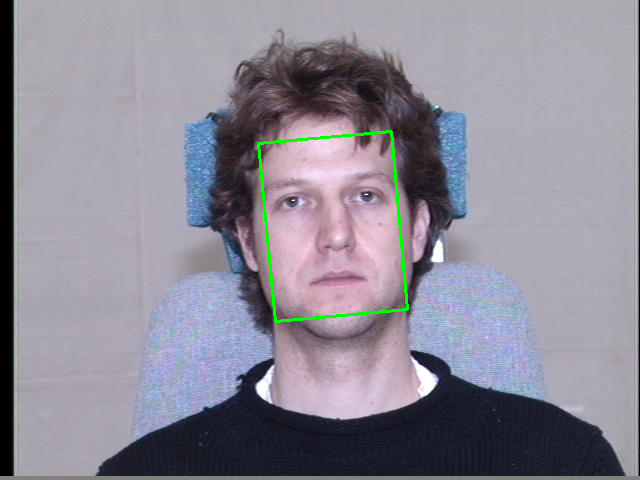
\includegraphics[trim=1.9in .7in 1.9in .5in, clip, height=1.0in]{../figures_pami/example.png} &
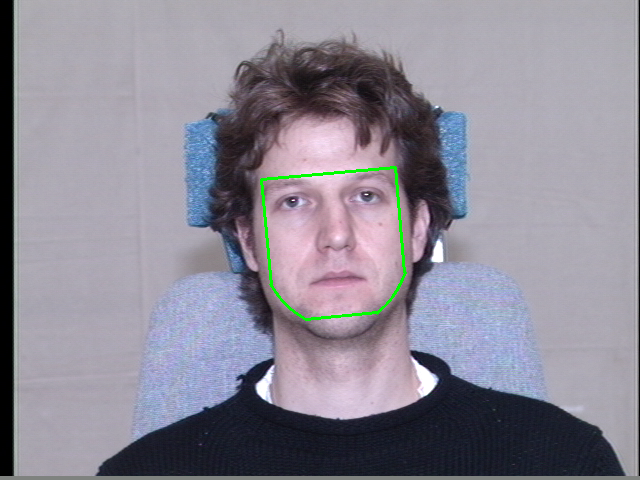
\includegraphics[trim=1.9in .7in 1.9in .5in, clip, height=1.0in]{../figures_pami/example_new.png} \\
Default window. & Proposed window.
\end{tabular}

{\tiny Recognition rates on the Multi-PIE database for
Algorithm 1 and [Yang2010-CVPR]}
\centerline{
\begin{tabular}{|c|c|c|c|c| }
\hline
Recognition rate & Session 2 & Session 3 & Session 4  \\
\hline
{Alg. 1, $S=1$} & 90.7\% & 89.6\% & 87.5\% \\
\hline
{Alg. 1} & 93.9\% & 93.8\% & 92.3\% \\
\hline
{Alg. 1 with improved window} & 95.0\% & {\bf 96.3}\% & {\bf 97.3}\% \\
\hline
\cite{Yang2010-CVPR} & {\bf 95.2}\% & 93.4\% & 95.1\% \\
\hline
\end{tabular}
} }

\subsection{Improved Occlusion Handling}
\frame{\tableofcontents[currentsection, currentsubsection]}

\frame{ \frametitle{Difficulty with MRF Model} 
MRF showed improved occlusion handling for the aligned case.
Unfortunately, when MRF model and iterative alignment are combined,
alignment stability problems arise.  The core problem: the algorithm
is unable to differentiate between the error caused by occlusion and
the error caused by initial misalignment. 
}

\frame{ \frametitle{Overlapping Block Model} 
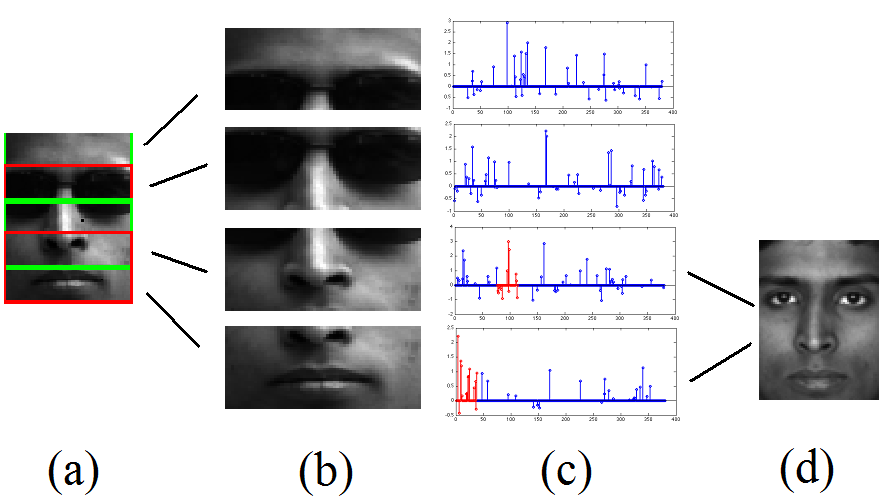
\includegraphics[width=4in]{../figures_pami/occ_block.png}
In order to better handle sunglasses, try overlapping Block Model: 
Perform recognition on a set of reduced size windows (Blocks) that are:
\begin{itemize}
\item small enough to sometimes miss occlusions
\item large enough to converge independently
\end{itemize}
...and vote to complete the classification.
}

\newcommand{\tempwidth}{0.1667\textwidth}
\frame{ \frametitle{Robustness to Sunglasses} 
\centering
\begin{tabular}{@{}c@{}c@{}c@{}c@{}c@{}c@{}}
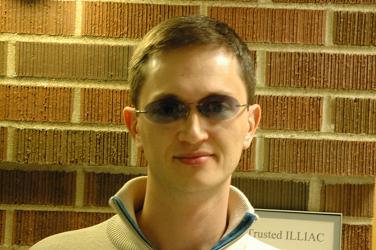
\includegraphics[width=\tempwidth,clip=true]{../figures_pami/uiuc_example/sunglasses/DSC_1565.JPG} &
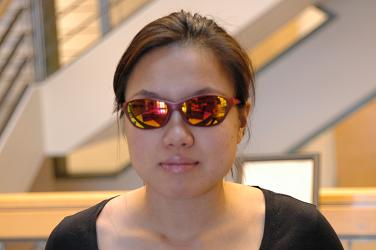
\includegraphics[width=\tempwidth,clip=true]{../figures_pami/uiuc_example/sunglasses/DSC_3656.JPG} &
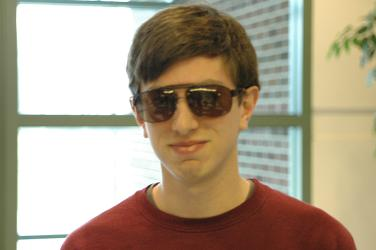
\includegraphics[width=\tempwidth,clip=true]{../figures_pami/uiuc_example/sunglasses/DSC_3827.JPG} &
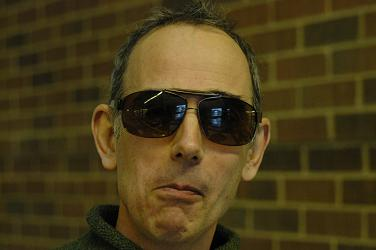
\includegraphics[width=\tempwidth,clip=true]{../figures_pami/uiuc_example/sunglasses/DSC_4090.JPG} &
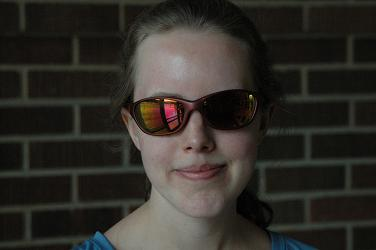
\includegraphics[width=\tempwidth,clip=true]{../figures_pami/uiuc_example/sunglasses/DSC_4106.JPG} &
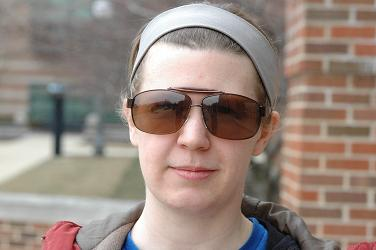
\includegraphics[width=\tempwidth,clip=true]{../figures_pami/uiuc_example/sunglasses/DSC_4126.JPG} \\
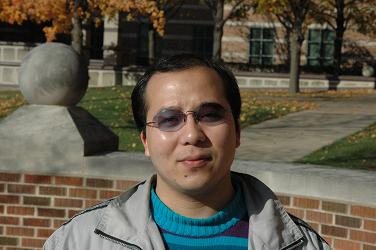
\includegraphics[width=\tempwidth,clip=true]{../figures_pami/uiuc_example/sunglasses_failed/DSC_1611.JPG} &
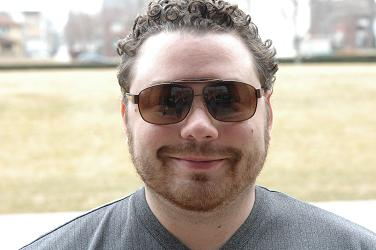
\includegraphics[width=\tempwidth,clip=true]{../figures_pami/uiuc_example/sunglasses_failed/DSC_3528.JPG} &
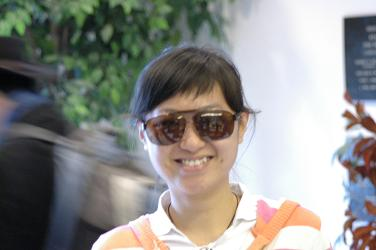
\includegraphics[width=\tempwidth,clip=true]{../figures_pami/uiuc_example/sunglasses_failed/DSC_3744.JPG} &
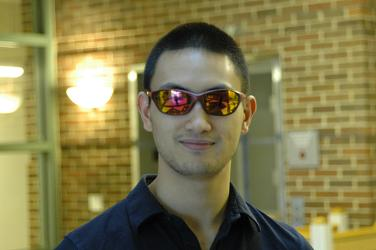
\includegraphics[width=\tempwidth,clip=true]{../figures_pami/uiuc_example/sunglasses_failed/DSC_3995.JPG} &
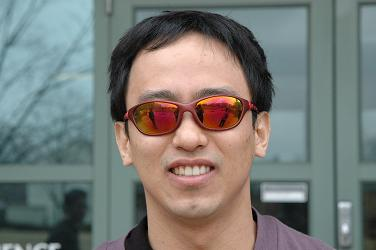
\includegraphics[width=\tempwidth,clip=true]{../figures_pami/uiuc_example/sunglasses_failed/DSC_4030.JPG} &
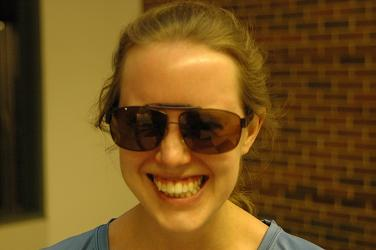
\includegraphics[width=\tempwidth,clip=true]{../figures_pami/uiuc_example/sunglasses_failed/DSC_4095.JPG} \\
\end{tabular}
Top row: examples where the overlapping blocks method succeeded. 
Bottom row: examples where the overlapping blocks method failed.
}


\subsection{Updated Experiments on Large Datasets}
\frame{\tableofcontents[currentsection, currentsubsection]}

\frame{\frametitle{Large Scale Experiments on Multi-PIE}
{\tiny Recognition rates on the Multi-PIE database for
different pairings of alignment and recognition stages.}
\tiny{ \centerline{
\begin{tabular}{|c|c|c|c|c|c|c|c|c|c|c| }
\hline
\backslashbox{Rec.}{Align.}
& \multicolumn{3}{|c|}{Face Detector}
& \multicolumn{3}{|c|}{Manual}
& \multicolumn{3}{|c|}{Iterative Alignment}
\\
\hline
Session $\rightarrow$	& 2		&3			&4			& 2		&3			&4			& 2		&3			&4		\\
\hline
NS	& 30.8\%	& 29.4\%	& 24.6\%	& 77.6\%	& 74.3\%	& 73.4\%	& 84.5\%	& 82.3\%	& 81.4\% \\
\hline
NN	& 26.4\%	& 24.7\%	& 21.9\%	& 67.3\%	& 66.2\%	& 62.8\%	& 73.5\%	& 69.6\%	& 69.3\% \\
\hline
LDA	& 5.1\%		& 5.9\%		& 4.3\%		& 49.4\%	& 44.3\%	& 47.9\%	& 91.0\%	& 89.9\%	& 88.1\% \\
\hline
LBP	& 39.9\%	& 38.1\%	& 33.9\%	& 93.3\%	& 91.2\%	& 92.9\%	& {\bf 95.2\%}	& {\bf 94.7\%}	& {\bf 93.5\%} \\
\hline
SRC	& -- & -- & -- & -- & -- & -- & 93.9\%	& 93.8\%	& 92.3\% \\
\hline
\end{tabular}
}} %centerline small
A combination of iterative alignment and LBP achieves highest recognition rate.
}

\frame{ \frametitle{Comparisons with LBP} 
\centerline{
\begin{tabular}{@{}cc@{}}
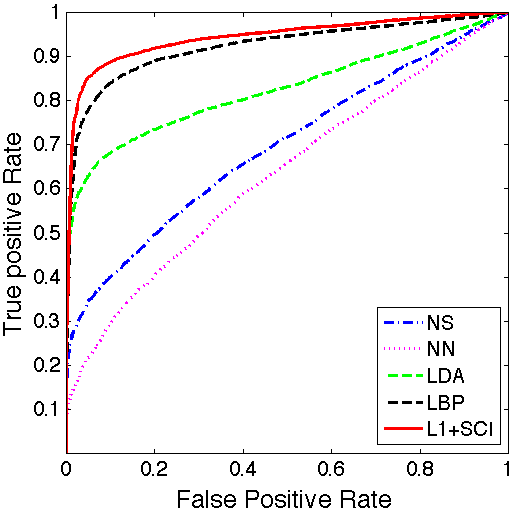
\includegraphics[height=2.0in]{../figures_pami/pami_roc_revision2} &
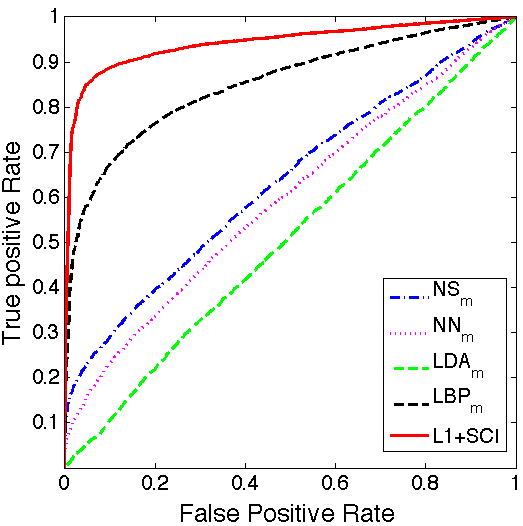
\includegraphics[height=2.0in]{../figures_pami/pami_roc2} \\
(a) & (b) \\
\end{tabular}
}
\small {\bf ROC curves} for subject validation on Multi-PIE database,
(a) for all algorithms with iterative alignment, and
(b) for the classical algorithms with manual alignment (indicated by a subscript ``m'').
}

\frame{ \frametitle{Improved performance on private dataset}
Recognition rates on a more realistic private database.

{\tiny
\begin{tabular}{|c|c|c|c|c|}
\hline
Test Category & C1 & C2 & C3 & C4  \\
\hline
\hline
Recognition Rate & 98.4\% & 95.8\% & 95.1\% & 40.9\% \\
\hline
\end{tabular}
}
}

